\documentclass[
11pt, % The default document font size, options: 10pt, 11pt, 12pt
codirector, % Uncomment to add a codirector to the title page
]{simple_charter}

% El títulos de la memoria, se usa en la carátula y se puede usar el cualquier
% lugar del documento con el comando \ttitle
\titulo{Master test plan: Sistema de SLAM Visual/Inercial}

% Nombre del posgrado, se usa en la carátula y se puede usar el cualquier lugar
% del documento con el comando \degreename
\posgrado{Carrera de Especialización en Sistemas Embebidos}

% Tu nombre, se puede usar el cualquier lugar del documento con el comando
% \authorname
\autor{Ing. Gonzalo Gabriel Fernández}

%\documentname{Master test plan}

% El nombre del director y co-director, se puede usar el cualquier lugar del
% documento con el comando \supname y \cosupname y \pertesupname y \pertecosupname
\director{Dr. Ing. Fabio Ardiani}
\pertenenciaDirector{Nimble One}

%\codirector{John Doe} % para que aparezca en la portada se debe descomentar la
% opción codirector en el documentclass
%\pertenenciaCoDirector{FIUBA}

% Nombre del cliente, quien va a aprobar los resultados del proyecto, se puede
% usar con el comando \clientename y \empclientename
\cliente{Ing. Leandro Borgnino}
\empresaCliente{Fundación Fulgor}

% Nombre y pertenencia de los jurados, se pueden usar el cualquier lugar del
% documento con el comando \jurunoname, \jurdosname y \jurtresname y
% \perteunoname, \pertedosname y \pertetresname.
\juradoUno{Nombre y Apellido (1)}
\pertenenciaJurUno{pertenencia (1)}
\juradoDos{Nombre y Apellido (2)}
\pertenenciaJurDos{pertenencia (2)}
\juradoTres{Nombre y Apellido (3)}
\pertenenciaJurTres{pertenencia (3)}

\fechaINICIO{24 de agost de 2023}		%Fecha de inicio de la cursada de GdP \fechaInicioName
\fechaFINALPlan{14 de octubre de 2023} 	%Fecha de final de cursada de GdP
\fechaFINALTrabajo{15 de mayo de 2024}	%Fecha de defensa pública del trabajo final

\begin{document}

\maketitle
\thispagestyle{empty}
\pagebreak

\thispagestyle{empty}
{\setlength{\parskip}{0pt}
\setcounter{tocdepth}{2}
\tableofcontents{}
}
\pagebreak

\section*{Registros de cambios}
\label{sec:registros-de-cambios}

\begin{table}[ht]
\label{tab:registro}
\centering
\begin{tabularx}{\linewidth}{@{}|c|X|c|@{}}
\hline
\rowcolor[HTML]{C0C0C0}
Revisión &
\multicolumn{1}{c|}{\cellcolor[HTML]{C0C0C0}Detalles de los cambios realizados}
& Fecha
\\ \hline
0 & Creación del documento & 15 de octubre de 2023 \\ \hline
1 & Detalle de tests para el subsistema A & 16 de octubre de 2023 \\ \hline
\end{tabularx}
\end{table}

\pagebreak

\section{1. Introducción}
\label{sec:1-introduccion}

En el presente documento se detalla la elección de estrategias de testing para el software
desarrollado para el sistema de odometría visual-inercial basado en SLAM propuesto en la planificación presentada en el documento [PYPH-DOC-001-R4], con el objetivo de
concientizar a todos los actores vinculados con el proyecto sobre los riesgos que deben cubrirse y
acordar cuántas pruebas deben realizarse y cuándo dentro del proceso de desarrollo de software.

Como se describe en el documento de arquitectura de software del sistema [PYPH-DOC-003-R2], el
software del sistema puede dividirse en los siguientes módulos:

\begin{itemize}
	\item Driver de la Unidad de Medición Inercial (IMU por sus siglas en  inglés), con el que se
	obtienen las lecturas del acelerómetro, giróscopo y magnetómetro y se transfieren a la aplicación.
	\item Driver de la cámara fotográfica, con el que se obtienen las imágenes de la cámara
	fotográfica y se transfieren a la aplicación.
	\item Algoritmo de SLAM, con el que se procesan los datos obtenidos con la IMU y la
	cámara fotográfica y se obtiene como salida un mapa del entorno, la posición y la orientación del
	sistema físco.
	\item Capa de comunicación con micro-ROS, con el que se transmiten los datos adquiridos con el
	sistema SLAM a un sistema externo de control, mediante la publicación en el canal de comunicación
	correspondiente del sistema ROS 2.
\end{itemize}

En la figura \ref{fig:software-arch} se observa un diagrama de bloques presentado en el documento de
arquitectura de software mencionado previamente, obtenido mediante la segmentación del proceso.

\begin{figure}[ht]
	\centering
	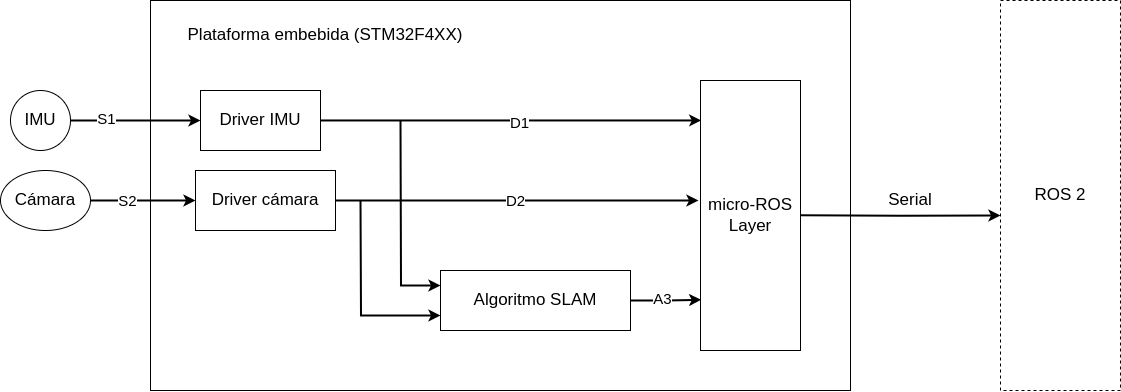
\includegraphics[width=\textwidth]{imgs/polyphemus_pipeline.png}
	\caption{Arquitectura de software de sistema SLAM}
	\label{fig:software-arch}
\end{figure}

En las siguientes secciones del documento, se selecciona las carcterísticas de calidad e evaluar
mediante  el testing del software desarrollado, se determina la importancia relativa de dichas
características y se define que características serán evaluadas en cada nivel de testing a realizar.
Además, se  divide el software en subsistemas, siguiendo el diagrama de la figura
\ref{fig:software-arch}, se determina la importancia relativa de cada uno y cuál será la técnica de
test a emplear en cada uno.

\section{2. Asignaciones}
\label{sec:2-asignaciones}

\subsection{Responsable}
\label{ssec:responsable}

El \textbf{responsable} de la elaboración del documento es el Ing. Gonzalo Gabriel Fernandez,
también a cargo del desarrollo del proyecto.

\subsection{Contratista}
\label{ssec:contratista}

El Ing. Gonzalo Gabriel Fernandez también toma el rol de \textbf{contratista} a cargo del testing
del software elaborado para el sistema SLAM.

\subsection{Alcance}
\label{ssec:alcance}

El alcance del test de aceptación es:

\begin{itemize}
	\item El driver de la Unidad de Medición Inercial
	\item El driver de la cámara fotográfica
	\item El algoritmo de SLAM
	\item La capa de comunicación con micro-ROS
\end{itemize}

\subsection{Objetivos}
\label{ssec:objetivos}

Los objetivos son:

\begin{itemize}
	\item Determinar si el sistema cumple los requerimientos
	\item Reportar y documentar las diferencias entre el comportamiento observado y el
	comportamiento esperado.
	\item Obtener una plataforma de testing que pueda ser reutilizada en futuras releases del
	proyecto.
\end{itemize}

\subsection{Precondiciones (externas)}
\label{ssec:precondiciones-externas}

Las precondiciones son:

\begin{itemize}
	\item El documento de requerimientos de software debe estar completo el mes posterior a la fecha
	de inicio del proyecto.
	\item La plataforma de testing estático, chequeo autómatico de código, generación automática de
	documentación debe ser funcional el mes posterior a la fecha de entraga del documento de
	requerimientos de software.
	\item Los tests deben estar finalizados el 26 de Enero de 2024.
\end{itemize}

\subsection{Precondiciones (internas)}
\label{ssec:precondiciones-internas}

Se necesitan las siguientes precondiciones para que las tareas de testing sean concluidas en tiempo
y forma:

\begin{itemize}
	\item El desarrollo y posterior ejecución de un test se lleva a cabo una vez finalizada la
	documentación del software involucrado.
	\item Todas las demoras en el desarrollo de tests deben ser documentadas y comunicadas al equipo
	de desarrollo.
	\item  Todos los cambios sobre un test serán documentados.
	\item Todas las herramientas e infraestructura necesaria para testing estará disponible durante
	el tiempo asignado a ejecucón de los tests.
\end{itemize}

\section{3. Bases del testing}
\label{sec:3-bases-del-testing}

Los tests detallados tienen como base los siguientes documentos:

\begin{itemize}
	\item \textbf{[PYPH-DOC-001-R4]:} Planificación de proyecto: Sistema de SLAM Visual/Inercial
	\item \textbf{[PYPH-DOC-002-R2]:} Especificación de requerimientos de software: Sistema de SLAM
	Visual/Inercial
	\item \textbf{[PYPH-DOC-003-R2]:} Arquitectura de software: Sistema de SLAM Visual/Inercial
\end{itemize}

\section{4. Estrategia de testing}
\label{sec:4-estrategia-de-testing}

\subsection{Selección de características de calidad}
\label{ssec:seleccion-de-caracteristicas-de-calidad}

La tabla \ref{tab:qualty-char} expone las características de calidad que deben ser evaluadas
y su importancia relativa (IR).

\begin{table}[ht]
\centering
\begin{tabular}{@{}lll@{}}
\toprule
\textbf{Características de calidad} & \textbf{Subcaracterística} & \textbf{IR (\%)} \\ \midrule
Funcionalidad & Idoneidad e interoperabilidad & 30 \\
Usabilidad & Comprensibilidad y operabilidad & 20 \\
Mantenibilidad & Posibilidad de cambiar y testeabilidad & 30 \\
Portabilidad & Adaptabilidad & 20 \\
Total & & 100 \\ \bottomrule
\end{tabular}
\caption{Importancia relativa de las características de calidad}
\label{tab:qualty-char}
\end{table}

A continuación se detallan las subcaracterísticas de calidad seleccionadas:

\begin{itemize}
	\item Idoneidad (\textit{Suitability}): las funcionalidades que provee el software deben ser las
	necesarias para que el sistema cumpla con todos los requisitos de funcionamiento establecidos en
	el documento [PYPH-DOC-002-R2].
	\item Interoperabilidad (\textit{Inteoperability}): los distintos módulos del software deben ser
	independientes y proveer interfaces claras y documentadas, de tal forma de permitir su
	reutilización en el proyecto actual, proyectos futuros o proyectos de terceros.
	\item Comprensibilidad (\textit{Understandability}): los distintos módulos del software y sus
	interfaces deben estar documentados de forma clara con ejemplos de uso que permitan al usuario
	adaptarlos a su sistema.
	\item Operabilidad (\textit{Operability}): un usuario con conocimientos en ROS 2 debe poder
	interactuar con el sistema rápidamente una vez interpretada la documentación del software del
	proyecto.
	\item Posibilidad de cambiar (\textit{Changeability}): tratándose de un proyecto que tendrá como
	usuario investigadores, es importante que el proyecto pueda ser modificado y extendido. Por lo
	tanto, el software debe estar completamente documentado y debe poseer ejemplos de extensión o uso
	de módulos de forma independiente.
	\item Testeabilidad (\textit{Testability}): el software debe ser desarrollo con un constante foco
	en su capacidad para evaluarlo.
	\item Adaptabilidad (\textit{Adaptability}):  se desea que el software sea portable a otras
	plataformas embebidas, y por lo tanto deben existir interfaces claras para portabilidad.
\end{itemize}

\subsection{Asignación de las características de calidad a cada nivel de prueba}
\label{ssec:asignacion-de-las-caracteristicas-de-calidad-a-cada-nivel-de-prueba}

A continuación se indica las características de calidad y su importancia relativa para cada nivel de
testing.

\subsubsection{Test unitario}
\label{sssec:test-unitario}

\begin{table}[H]
\centering
\begin{tabular}{@{}lc@{}}
\toprule
\textbf{Características de calidad} & \textbf{Importancia relativa (\%)} \\ \midrule
Posibilidad de cambiar              & 40                                 \\
Testeabilidad                       & 60                                 \\
Total                               & 100                                \\ \bottomrule
\end{tabular}
\caption{Importancia de las características de calidad en el test unitario}
\label{tab:ir-unit}
\end{table}

\subsubsection{Test de integración de software}
\label{sssec:test-de-integracion-de-software}

\begin{table}[H]
\centering
\begin{tabular}{@{}lc@{}}
\toprule
\textbf{Características de calidad} & \textbf{Importancia relativa (\%)} \\ \midrule
Interoperabilidad                   & 10                                 \\
Comprensibilidad                    & 20                                 \\
Posibilidad de cambiar              & 10                                 \\
Testeabilidad                       & 30                                 \\
Adaptabilidad                       & 30                                 \\
Total                               & 100                                \\ \bottomrule
\end{tabular}
\caption{Importancia de las características de calidad en el test de integración de software}
\label{tab:ir-int-soft}
\end{table}

\subsubsection{Test de integración de software con hardware}
\label{sssec:test-de-integracion-de-software-con-hardware}

\begin{table}[H]
\centering
\begin{tabular}{@{}lc@{}}
\toprule
\textbf{Características de calidad} & \textbf{Importancia relativa (\%)} \\ \midrule
Idoneidad                           & 20                                 \\
Comprensibilidad                    & 30                                 \\
Posibilidad de cambiar              & 5                                  \\
Testeabilidad                       & 5                                  \\
Adaptabilidad                       & 40                                 \\
Total                               & 100                                \\ \bottomrule
\end{tabular}
\caption{Importancia de las características de calidad en el test de integración de software con
hardware}
\label{tab:ir-int-soft-hard}
\end{table}

\subsubsection{Test de sistema}
\label{sssec:test-de-sistema}

\begin{table}[H]
\centering
\begin{tabular}{@{}lc@{}}
\toprule
\textbf{Características de calidad} & \textbf{Importancia relativa (\%)} \\ \midrule
Idoneidad                           & 50                                 \\
Comprensibilidad                    & 20                                 \\
Operabilidad                        & 30                                 \\
Total                               & 100                                \\ \bottomrule
\end{tabular}
\caption{Importancia de las características de calidad en el test de sistema}
\label{tab:ir-test-sys}
\end{table}

\subsubsection{Test de aceptación}
\label{sssec:test-de-aceptacion}

\begin{table}[H]
\centering
\begin{tabular}{@{}lc@{}}
\toprule
\textbf{Características de calidad} & \textbf{Importancia relativa (\%)} \\ \midrule
Idoneidad                           & 60                                 \\
Operabilidad                        & 40                                 \\
Total                               & 100                                \\ \bottomrule
\end{tabular}
\caption{Importancia de las características de calidad en el test de aceptación}
\label{tab:ir-test-accept}
\end{table}

\subsubsection{Test de campo}
\label{sssec:test-de-campo}

\begin{table}[H]
\centering
\begin{tabular}{@{}lc@{}}
\toprule
\textbf{Características de calidad} & \textbf{Importancia relativa (\%)} \\ \midrule
Idoneidad                           & 60                                 \\
Operabilidad                        & 40                                 \\
Total                               & 100                                \\ \bottomrule
\end{tabular}
\caption{Importancia de las características de calidad en el test de campo}
\label{tab:ir-test-field}
\end{table}

\subsection{Asignación de niveles de prueba a las características de calidad}
\label{ssec:asignacion-de-niveles-de-prueba-a-las-caracteristicas-de-calidad}

En la tabla \ref{tab:test-level-quality} se observan los niveles de prueba asignados a las distintas
características de calidad detalladas en la sección
\ref{ssec:asignacion-de-las-caracteristicas-de-calidad-a-cada-nivel-de-prueba}.

\begin{table}[H]
\centering
\begin{tabular}{@{}llllllll@{}}
\toprule
\textbf{} & \textbf{(1)} & \textbf{(2)} & \textbf{(3)} & \textbf{(4)} & \textbf{(5)} & \textbf{(6)} & \textbf{(7)} \\ \midrule
\textbf{Importancia relativa (\%)} & 15 & 15 & 10 & 10 & 10 & 20 & 20 \\
\textbf{Test unitario} &  &  &  &  & ++ & ++ &  \\
\textbf{\begin{tabular}[c]{@{}l@{}}Test de integración de software\end{tabular}}
 &  & ++ & ++ &  & ++ & ++ & ++ \\
\textbf{Test de integración de software y hardware} & + &  & ++ &  & + & + & ++ \\
\textbf{Test de sistema} & + &  & + & ++ &  &  &  \\
\textbf{Test de aceptación} & ++ &  &  & ++ &  &  &  \\
\textbf{Test de campo} & ++ &  &  & ++ &  &  &  \\ \bottomrule
\end{tabular}
\caption{Asignación de nivel de test por característica de calidad}
\label{tab:test-level-quality}
\end{table}

Donde los números corresponden a las siguientes características de calidad:
\begin{enumerate}
	\item Idoneidad
	\item Interoperabilidad
	\item Comprensibilidad
	\item Operabilidad
	\item Posibilidad de cambiar
	\item Testeabilidad
	\item Adaptabilidad
\end{enumerate}

Donde las simbología representa lo siguiente:
\begin{itemize}
	\item ++ : la característica de calidad será cubierta completamente ya que es un objetivo
	importante en ese nivel de testing.
	\item + : el nivel de testing cubrirá la característica de calidad.
	\item vacío: la característica de calidad no es un problema en ese nivel de testing
\end{itemize}

Los motivos de la asignación de niveles de prueba a las características de calidad seleccionadas son
los siguientes:

\begin{itemize}
	\item Idoneidad: es importante en la integración de software con hardware, en las pruebas de
	sistema, en las pruebas de aceptación y en las pruebas de campo, donde se comprueba que
	efectivamente el software desarrollado cumple los requerimientos planteados en el documento de
	ERS [PYPH-DOC-002-R2].
	\item Interoperabilidad: en el test de integración de software es donde se comprobará la
	independencia de los distintos módulos que componen el sistema, la arquitectura de sus
	interfaces y su documentación.
	\item Comprensibilidad: será evaluada principalmente en la integración de software, en la
	integración de software con hardware y en las pruebas de sistema, poniendo foco en la experiencia
	del usuario al utilizar el software.
	\item Operabilidad: en las pruebas de sistema se analiza la interacción con el sistema externo
	con ROS 2, y se evaluará la facilidad de uso del sistema.
	\item Posibilidad de cambiar: será foco en las pruebas unitarias y en la integración de software
	analizando la claridad y escalabilidad del software desarrollado.
	\item Testeabilidad: especialmente importante a bajo nivel, en las pruebas unitarias y de
	integración de software. Es imprescindible que el software desarrollado sea fácil de evaluar y
	compatible con una plataforma de testing automático.
	\item Adaptabilidad: en las pruebas de integración de software e integración de software con
	hardware es donde se evaluará la facilidad de portación a otras arquitecturas de procesador y
	otros sistemas embebidos.
\end{itemize}

\section{5. Estrategias por nivel de prueba}
\label{sec:5-estrategias-por-nivel-de-prueba}

A continuación, se divide elsistema en subsistemas, se les asigna una importancia relativa y se
define la importancia de las característica de calidad en cada uno de ellos.
Para finalizar, se define qué técnicas de test serán utilizadas en cada subsistema.

\subsection{División del sistema en subsistemas}
\label{ssec:division-del-sistema-en-subsistemas}

El software del sistema SLAM puede dividirse en los siguientes subsistemas:

\begin{itemize}
	\item \textbf{Subsistema A: driver de la IMU}, con el que se obtienen las lecturas del acelerómetro, giróscopo y magnetómetro y se transfieren a la aplicación.
	\item \textbf{Subsistema B: driver de la cámara fotográfica}, con el que se obtienen las imágenes de la cámara fotográfica y se transfieren al módulo de procesamiento de imágenes.
	\item \textbf{Subsistema C: algoritmo de SLAM}, con el que se procesan los datos obtenidos de la
	IMU y la cámara fotográfica y se obtiene como salida un mapa del entorno, la posición y la
	orientación del sistema físico.
	\item \textbf{Subsistema D: capa de comunicación con micro-ROS}, con el que se transmiten los
	datos adquiridos con el sistema SLAM a un sistema externo de control, mediante la publicación
	en el canal de comunicación correspondiente del sistema ROS 2.
\end{itemize}

\subsection{Importancia relativa de los subsistemas}
\label{ssec:importancia-relativa-de-los-subsistemas}

En la tabla \ref{tab:ir-subsys} se observa la importancia relativa asignada a cada subsistema
del proyecto.

\begin{table}[ht]
\centering
\begin{tabular}{@{}lc@{}}
\toprule
Subsistema & Importancia relativa (\%) \\ \midrule
Driver de la IMU & 30 \\
Driver de la cámara fotográfica & 30 \\
Algoritmo de SLAM & 30 \\
Capa de comunicación con micro-ROS & 10 \\
Total & 100 \\ \bottomrule
\end{tabular}
\caption{Importancia relatica de los subsistemas}
\label{tab:ir-subsys}
\end{table}

\subsection{Importancia de test por combinación de subsistema y característica de calidad}
\label{ssec:importancia-de-test-por-combinacion-de-subsistema-y-caracteristica-de-calidad}

En la tabla \ref{tab:quality-subsys} se observa la importancia de cada característica de
calidad seleccionada en cada subsistema en específico.

\begin{table}[ht]
\centering
\begin{tabular}{@{}lllll@{}}
\toprule
 & Sub. A & Sub. B & Sub. C & Sub. D \\ \midrule
\rowcolor[HTML]{EFEFEF}
Importancia relativa (\%) & 30 & 30 & 30 & 10 \\
Idoneidad & ++ & ++ & ++ & + \\
Interoperabilidad & ++ & ++ & + &  \\
Comprensibilidad & ++ & ++ & + &  \\
Operabilidad &  &  &  & ++ \\
Posibilidad de cambiar & + & + & ++ & + \\
Testeabilidad & ++ & ++ & ++ &  \\
Adaptabilidad & ++ & ++ & + &  \\ \bottomrule
\end{tabular}
\caption{Importancia de características de calidad en cada subsistema}
\label{tab:quality-subsys}
\end{table}

Donde las simbología representa lo siguiente:
\begin{itemize}
	\item ++ : La característica de calidad será cubierta completamente ya que es un objetivo
	importante en ese subsistema.
	\item + : La característica de calidad se cubrirá en el subsistema.
	\item vacío: La característica de calidad no es necesaria en el subsistema.
\end{itemize}

\subsection{Técnicas de test a ser utilizadas}
\label{ssec:tecnicas-de-test-a-ser-utilizadas}

Las técnicas de test a utilizar son:

\begin{itemize}
	\item \textit{Elementary Comparison Test} (ECT)
	\item \textit{Classification-Tree Method} (CTM)
	\item \textit{Control Flow Test} (CFT)
	\item \textit{State Transition Testing} (STT)
\end{itemize}

Se aplicarán la técnicas de test mencionadas a cada uno de los subsistemas, de acuerdo a las tabla
\ref{tab:tec-subsys}.

\begin{table}[H]
\centering
\begin{tabular}{@{}lcccc@{}}
\toprule
Técnica de test & Sub. A & Sub. B & Sub. C & Sub. D \\ \midrule
ECT &   & + &  &  \\
CTM &  &  & + &  \\
CFT & + & + & + & + \\
STT & + &  &  & + \\ \bottomrule
\end{tabular}
\caption{Técnicas de test a aplicar en cada subsistema}
\label{tab:tec-subsys}
\end{table}

\pagebreak
\section{6. Test de subsistema A: driver de la IMU}
\label{sec:6-test-de-subsistema-a-driver-de-la-imu}

\subsection{Test unitario}
\label{ssec:test-unitario}

El test unitario del diver de la IMU se realiza mediante \textit{Control Flow Test},
controlando principalmente los mensajes de error y éxito retornado por las distintas funciones
que lo componen.

\subsection{Test de sistema}
\label{ssec:test-de-sistema}

A continuación se detallan los test de sistema a realizar para el software vinculado a la IMU.

\subsubsection{Máquina de estados finitos (FSM) de interacción con la IMU}
\label{sssec:maquina-de-estados-finitos-fsm-de-interaccion-con-la-imu}

En la figura \ref{fig:fsm-de-interaccion-con-la-imu} se observa la máquina de estados finitos
que utilizada para interactuar con la IMU y sobre la que aplicará la técnica de \textit{State
Transition Testing}.

\begin{figure}[H]
\centering
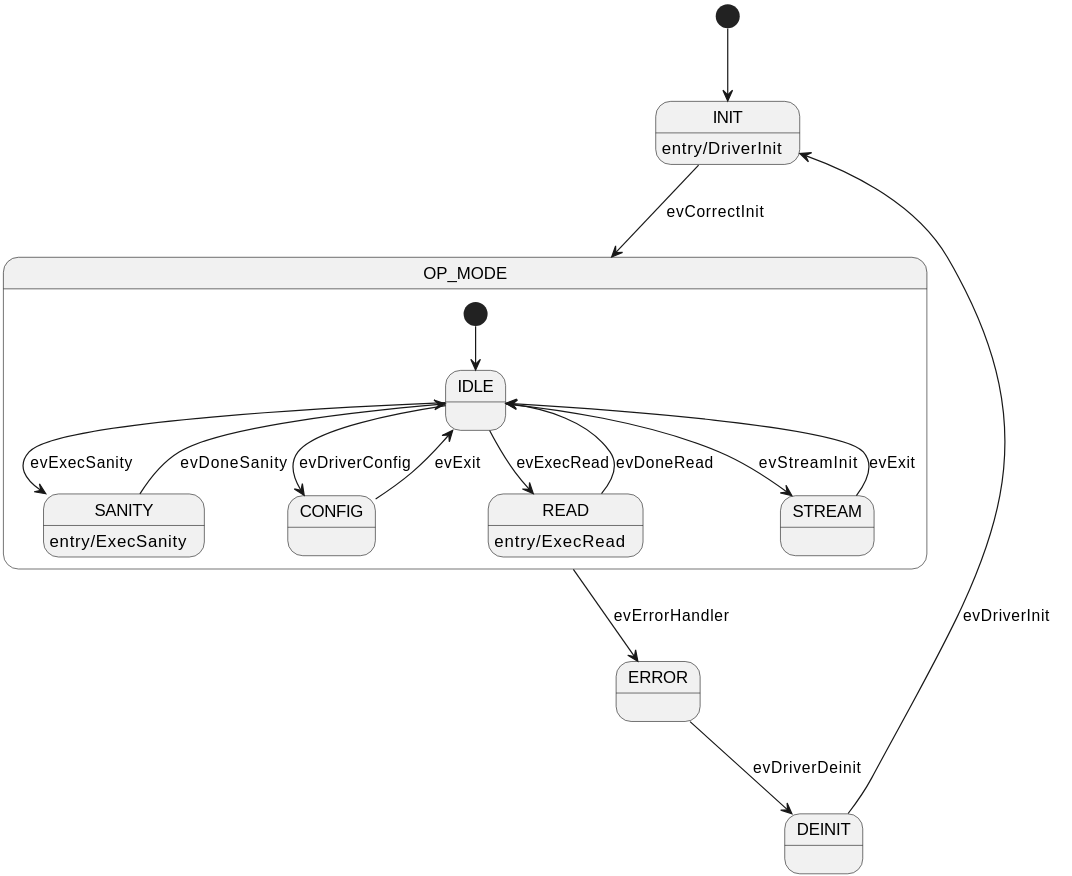
\includegraphics[width=\textwidth]{imgs/imu_bridge_fsm.png}
\caption{FSM de interacción con la IMU}
\label{fig:fsm-de-interaccion-con-la-imu}
\end{figure}


\begin{landscape}
\subsubsection{Tabla de estados y eventos}
\label{sssec:tabla-de-estados-y-eventos}

A partir de la máquina de estados de la figura \ref{fig:fsm-de-interaccion-con-la-imu} se obtiene
la tabla \ref{tab:imu-fsm-estados-y-eventos} de estados y eventos, donde se observa tanto las
transiciones legales como ilegales.

\begin{table}[ht]
\centering
\begin{tabular}{|
>{\columncolor[HTML]{EFEFEF}}c |c|c|c|c|c|c|c|c|}
\hline
 & \cellcolor[HTML]{EFEFEF}\textbf{INIT} & \cellcolor[HTML]{EFEFEF}\textbf{IDLE} & \cellcolor[HTML]{EFEFEF}\textbf{SANITY} & \cellcolor[HTML]{EFEFEF}\textbf{CONFIG} & \cellcolor[HTML]{EFEFEF}\textbf{READ} & \cellcolor[HTML]{EFEFEF}\textbf{STREAM} & \cellcolor[HTML]{EFEFEF}\textbf{ERROR} & \cellcolor[HTML]{EFEFEF}\textbf{DEINIT} \\ \hline
evCorrectInit & 1. IDLE & \textbullet & \textbullet & \textbullet & \textbullet & \textbullet & \textbullet & \textbullet \\ \hline
evExecSanity & \textbullet & 2. SANITY & \textbullet & \textbullet & \textbullet & \textbullet & \textbullet & \textbullet \\ \hline
evDriverConfig & \textbullet & 3. CONFIG & \textbullet & \textbullet & \textbullet & \textbullet & \textbullet & \textbullet \\ \hline
evExecRead & \textbullet & 4. READ & \textbullet & \textbullet & \textbullet & \textbullet & \textbullet & \textbullet \\ \hline
evStreamInit & \textbullet & 5. STREAM & \textbullet & \textbullet & \textbullet & \textbullet & \textbullet & \textbullet \\ \hline
evDoneSanity & \textbullet & \textbullet & 7. IDLE & \textbullet & \textbullet & \textbullet & \textbullet & \textbullet \\ \hline
evExit & \textbullet & \textbullet & \textbullet & 9. IDLE & \textbullet & 13. IDLE & \textbullet & \textbullet \\ \hline
evDoneRead & \textbullet & \textbullet & \textbullet & \textbullet & 11. IDLE & \textbullet & \textbullet & \textbullet \\ \hline
evErrorHandler & \textbullet & 6. ERROR & 8. ERROR & 10. ERROR & 12.ERROR & 14. ERROR & \textbullet & \textbullet \\ \hline
evDriverDeinit & \textbullet & \textbullet & \textbullet & \textbullet & \textbullet & \textbullet & 15. DEINIT & \textbullet \\ \hline
evDriverInit & \textbullet & \textbullet & \textbullet & \textbullet & \textbullet & \textbullet & \textbullet & 16. INIT \\ \hline
\end{tabular}
\caption{Tabla de estados y eventos asociada a la FSM de interacción con la IMU}
\label{tab:imu-fsm-estados-y-eventos}
\end{table}
\end{landscape}

\subsubsection{Árbol de transiciones}
\label{sssec:arbol-de-transiciones}

A partir de la tabla \ref{tab:imu-fsm-estados-y-eventos} se puede general el árbol de transiciones
de la figura \ref{fig:arbol-de-transiciones}, donde se observan 9 caminos de test diferentes.

\begin{figure}[ht]
\centering
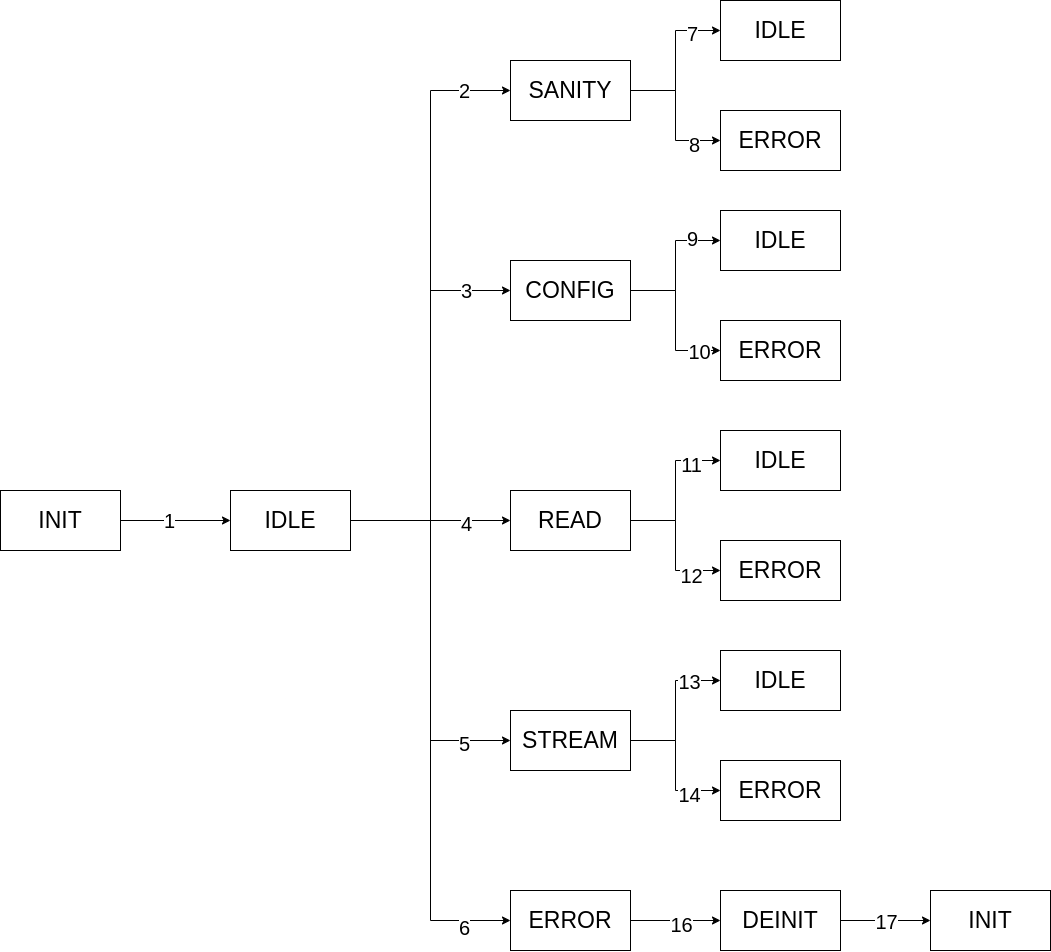
\includegraphics[width=0.9\textwidth]{imgs/imu_bridge_fsm-transition_tree.png}
\caption{Árbol de transiciones asociada a la FSM de interacción con la IMU}
\label{fig:arbol-de-transiciones}
\end{figure}

\subsubsection{Casos de prueba para la FSM}
\label{sssec:casos-de-prueba-para-la-fsm}

A partir del árbol de transiciones de la figura \ref{fig:arbol-de-transiciones} se obtiene la
tabla \ref{tab:fsm-imu-casos-legales} con todos los casos legales a cubrir y de la cual se puede
generar 9 scripts de test diferentes (L1 a L9) que seguirán la secuencia de eventos descripta.

\begin{table}[H]
\centering
\begin{tabular}{|c|c|c|c|}
\hline
\rowcolor[HTML]{EFEFEF}
\textbf{ID} & \textbf{Evento de entrada} & \textbf{Acción esperada} & \textbf{Estado esperado} \\ \hline
L1.1 & evCorrectInit & DriverInit & IDLE \\ \hline
L1.2 & evExecSanity & ExecSanity & SANITY \\ \hline
L1.3 & evDoneSanity &  & IDLE \\ \hline
\rowcolor[HTML]{EFEFEF}
L2.1 & evCorrectInit & DriverInit & IDLE \\ \hline
\rowcolor[HTML]{EFEFEF}
L2.2 & evExecSanity & ExecSanity & SANITY \\ \hline
\rowcolor[HTML]{EFEFEF}
L2.3 & evErrorHandler & ErrorFlag & ERROR \\ \hline
L3.1 & evCorrectInit & DriverInit & IDLE \\ \hline
L3.2 & evDriverConfig & RecvConfig & CONFIG \\ \hline
L3.3 & evExit &  & IDLE \\ \hline
\rowcolor[HTML]{EFEFEF}
L4.1 & evCorrectInit & DriverInit & IDLE \\ \hline
\rowcolor[HTML]{EFEFEF}
L4.2 & evDriverConfig & RecvConfig & CONFIG \\ \hline
\rowcolor[HTML]{EFEFEF}
L4.3 & evErrorHandler & ErrorFlag & ERROR \\ \hline
L5.1 & evCorrectInit & DriverInit & IDLE \\ \hline
L5.2 & evExecRead & ExecRead & READ \\ \hline
L5.3 & evDoneRead &  & IDLE \\ \hline
\rowcolor[HTML]{EFEFEF}
L6.1 & evCorrectInit & DriverInit & IDLE \\ \hline
\rowcolor[HTML]{EFEFEF}
L6.2 & evExecRead & ExecRead & READ \\ \hline
\rowcolor[HTML]{EFEFEF}
L6.3 & evErrorHandler & ErrorFlag & ERROR \\ \hline
L7.1 & evCorrectInit & DriverInit & IDLE \\ \hline
L7.2 & evStreamInit & StreamInit & STREAM \\ \hline
L7.3 & evExit &  & IDLE \\ \hline
\rowcolor[HTML]{EFEFEF}
L8.1 & evCorrectInit & DriverInit & IDLE \\ \hline
\rowcolor[HTML]{EFEFEF}
L8.2 & evStreamInit & StreamInit & STREAM \\ \hline
\rowcolor[HTML]{EFEFEF}
L8.3 & evErrorHandler & ErrorFlag & ERROR \\ \hline
L9.1 & evCorrectInit & DriverInit & IDLE \\ \hline
L9.2 & evErrorHandler & ErrorFlag & ERROR \\ \hline
L9.3 & evDriverDeinit & DriverDeinit & DEINIT \\ \hline
L9.4 & evDriverInit & DriverInit & INIT \\ \hline
\end{tabular}
\caption{Casos de prueba legales para la FSM de interacción con la IMU}
\label{tab:fsm-imu-casos-legales}
\end{table}

De la tabla \ref{tab:imu-fsm-estados-y-eventos} se puede generar los casos de prueba ilegales,
no descriptos en el documento por la cantidad de casos ilegales posibles.

% \begin{plantuml}
% @startuml
% [*] --> INIT

% INIT : entry/DriverInit
% INIT --> OP\_MODE : evCorrectInit

% state OP\_MODE {
%     [*] --> IDLE
%     IDLE --> SANITY : evExecSanity
%     IDLE --> CONFIG : evDriverConfig
%     IDLE --> READ : evExecRead
%     IDLE --> STREAM : evStreamInit

%     SANITY : entry/ExecSanity
%     SANITY --> IDLE : evDoneSanity

%     CONFIG --> IDLE : evExit

%     READ : entry/ExecRead
%     READ --> IDLE : evDoneRead

%     STREAM --> IDLE : evExit
% }

% OP\_MODE --> ERROR : evErrorHandler
% ERROR --> DEINIT : evDriverDeinit
% DEINIT --> INIT : evDriverInit
% @enduml
% \end{plantuml}


\subsection{Test de aceptación}
\label{ssec:test-de-aceptacion}

A continuación se detallan los test de aceptación a realizar en función de los requerimientos
planteados en el documento de especificación de requerimientos de software [PYPH-DOC-002-R2].

\subsubsection{Ensayo: Configuración de rango en sensor de la IMU}
\label{sssec:ensayo-configuracion-de-rango-en-sensor-de-la-imu}

[PYPH-RS-010] \textit{El sistema SLAM debe permitir mediante, un mensaje en el canal de comunicación
asociado de la IMU, configurar el rango de cada uno de los sensores que la componen, respetando las
opciones disponibles de rango en cada uno de ellos.}

\begin{itemize}
	\item \textbf{Estado inicial:} La comunicación con el sistema externo a través de ROS 2 se
	encuentra establecida. La configuración de la IMU es la dada por la inicialización.
	\item \textbf{Estado final:} El giróscopo de la IMU se encuentra configurado con un nuevo rango
	distinto al de la inicialización.
	\item \textbf{Secuencia de pasos:} Todas las acciones descriptas se ejecutan desde el sistema
	externo con ROS 2.
	\begin{enumerate}
		\item Listar servicios de ROS 2 disponibles.
		\item Revisar que se encuentre el servicio que permite leer el rango actual del giróscopo
		en base a la documentación del proyecto.
		\item Si el servicio no se encuentra el ensayo se considera fallido.
		\item Mediante el cliente asociado al sericio del punto 2, leer el rango actual del
		giróscopo.
		\item Revisar que se encuentre el servicio que permite configurar el rango del giróscopo
		en base a la documentación del proyecto.
		\item Si el servicio no se encuentra el ensayo se considera fallido.
		\item Mediante el cliente asociado al servicio del punto 5, enviar un rango de giróscopo
		inválido.
		\item Esperar error en la respuesta del servicio, de lo contrario el ensayo se considera
		fallido.
		\item Mediante el cliente asociado al servicio del punto 5, enviar un rango de giróscopo
		válido y diferente del obtenido en el punto 4.
		\item Esperar respuesta de configuración correcta de parte del servicio, de lo contrario se
		considera fallido.
		\item Si los pasos previos se realizaron con éxito el ensayo se considera cumplido.
	\end{enumerate}
\end{itemize}

Ensayos equivalentes para el resto de los sensores que componen la IMU.

\subsubsection{Ensayo: Generación de stream de datos con lecturas de sensor de la IMU}
\label{sssec:ensayo-generacion-de-stream-de-datos-con-lecturas-de-sensor-de-la-imu}

[PYPH-RS-017] \textit{El sistema SLAM debe permitir, mediante un mensaje en el canal de comunicación
asociado a la IMU, solicitar iniciar (y detener) un stream de lecturas en tiempo real de cada uno de
los sensores que la componen.}

\begin{itemize}
	\item \textbf{Estado inicial:} La comunicación con el sistema externo a través de ROS 2 se
	encuentra establecida. La configuración de la IMU es la dada por la inicialización.
	\item \textbf{Estado final:} El sistema externo inició y detuvo un stream de datos con las
	lecturas obtenidas con el giróscopo de la IMU.
	\item \textbf{Secuencia de pasos:} Todas las acciones descriptas se ejecutan desde el sistema
	externo con ROS 2.
	\begin{enumerate}
		\item Listar los topics de ROS 2 disponibles.
		\item Revisar que se encuentre el topic asociado al stream de datos con las lecturas de los
		tres ejes del giróscopo en base a la documentación del proyecto.
		\item Si el topic no se encuentra el ensayo se considera fallido.
		\item Realizar un echo (si es posible graficar mediante una herramienta como
		\textit{rqt\_graph}) del topic.
		\item Verificar que no se publican datos en el topic, de lo contrario el ensayo se considera
		fallido.
		\item Listar servicios de ROS 2 disponibles.
		\item Revisar que se encuentre el servicio que permite iniciar y detener un stream de datos
		con las lecturas de los tres ejes del giróscopo en base a la documentación del proyecto.
		\item Si el servicio no se encuentra el ensayo se considera fallido.
		\item Mediante el cliente asociado al sericio del punto 2, iniciar el stream de datos con
		las lecturas de los tres ejes del giróscopo.
		\item Realizar un echo (si es posible graficar mediante una herramienta como
		\textit{rqt\_graph}) del topic.
		\item Verificar que se publican datos y que se corresponden con los movimientos de la IMU
		al rotarla manualmente.
		\item Si los datos no se correponden con los movimientos de la IMU el ensayo se considera
		fallido.
		\item Mediante el cliente asociado al servicio del punto 2, detener el stream de datos con
		las lecturas de los tres ejes del giróscopo.
		\item Realizar un echo (si es posible graficar mediante una herramienta como
		\textit{rqt\_graph}) del topic.
		\item Verificar que no se publican datos en el topic, de lo contrario el ensayo se considera
		fallido.
		\item Si los pasos previos se realizaron con éxito el ensayo se considera cumplido.
	\end{enumerate}
\end{itemize}

Ensayos equivalentes para el resto de los sensores que componen la IMU.


\end{document}
